\header{
    \headtitle{Le hussard de la garde} \label{le-hussard-de-la-garde}
    %
    
    \insertComment{Publiée dans "Le panier aux ordures" comme "Manon" (1866).}{}
}

\enluminure{4}{\href{https://www.youtube.com/watch?v=Hi1PoPITPe0}{C}}{'était} un hussard de la garde,
\\Qui revenait de garnison
\\A Briançon,
\\Portant sa pine en hallebarde,
\\Agrémentée de deux roustons
\\Pleins de morpions.
\\\\\textbf{Refrain :}
\\Vivre sans soucis,
\\Boire du purin, manger de la merde:
\\C'est le seul moyen
\\De ne jamais mourir de faim.
\\Oh merde, merde divine,
\\Toi seule as des appâts.
\\La rose a des épines,
\\Toi, merde, tu n'en as pas.
\\\\En descendant la rue Troussecouille,
\\Il rencontra la garce Manon,
\\Qui pue du con.
\\Il lui dit: "Ma chaste fripouille,
\\Le régiment s'en va demain,
\\La pine en main."
\\\\En vain Manon se désespère,
\\De voir partir tous ses amis,
\\Avec leurs vits!
\\Elle va trouver Madame sa mère,
\\Lui dit: "Je veux partir aussi,
\\Sacrée chipie."
\breakpage
"Ma fille, ma sacrée garce de fille,
\\N'vas pas avec ce hussard là,
\\Il te perdra!
\\Ils t'ont fendue jusqu'au nombril,
\\Ils te fendront jusqu'au menton
\\La peau du con."
\\\\Ma mère, ma sacrée garce de mère,
\\Tous tes conseils tu peux, vois-tu, 
\\T'les foutr' au cul !
\\Ça te va vraiment d'faire des manières,
\\Alors que d'puis l'âge de 8 ans,
\\Tu suces des glands !
\\\\"Ma fille, ma sacrée putain d'fille,
\\Quand sera parti ce hussard là,
\\Tu te branleras.
\\Je t'achèterai une cheville,
\\Avec laquelle tu te masturberas
\\A tour de bras."
\\\\"Ma mère, mon vieux chameau de mère,
\\Quand tu me parles de me branler,
\\Tu me fais chier.
\\Un vit ça sort de l'ordinaire,
\\Ca vous laisse un doux souvenir
\\Qui vous fait jouir."
\\\\La garce s'est quand même laissée faire
\\Par le hussard qui la pressait
\\De se donner.
\\Il lui mit une si longue affaire
\\Que ça lui sortit par le nez,
\\Ca l'a tuée.
\breakpage
Manon, la sacrée garce est morte,
\\Morte comme elle avait vécu:
\\La pine au cul.
\\Le corbillard est à sa porte,
\\Traîné par quatre morpions en deuil,
\\La larme à l'oeil.
%Ils l'ont conduite au cimetière,
%\\Et sur sa tombe ils ont gravé
%\\Tous ces couplets.
%\\Mais le fossoyeur, par derrière,
%\\L'a déterrée, et l'a violée,
%\\Ca lui manquait.
\\\\L'auteur de cette barcarolle
\\Est un vrai hussard à chevrons,
\\Foutu cochon.
\\Quand il mourut de la vérole,
\\Les asticots qui l'ont bouffé
\\L'ont dégueulé.
\begin{center}
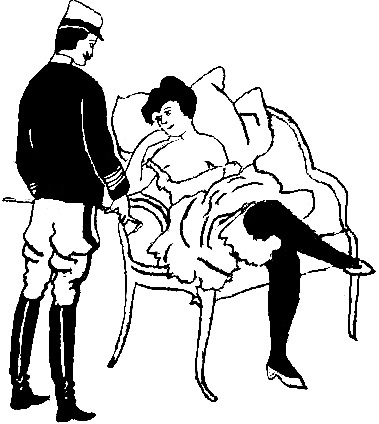
\includegraphics[width=0.8\textwidth]{images/hussard.jpg}
\end{center}

\breakpage